\section{Advection}

\subsection{Analytical Equation}

Advection is a bit of an exception as a hydrodynamics method because we're not actually solving the (ideal) gas equations, but these instead:

\begin{equation}
	\DELDT{ \U } + \V \cdot \DELDX{\U} = 0
\end{equation}


Which is still a conservation law of the form

\begin{equation}
	\DELDT{ \U } + \DELDX{\F} = 0
\end{equation}

with the flux tensor 

\begin{equation}
	\F = \V \cdot \U
\end{equation}

We assume $\V = $ const.

The analytical solution is given by any function $q(x)$ with $\U(x,t) = q(\x - \V t)$, which is just $q(x)$ translated by $\V t$.




\subsection{Piecewise Constant Method}

\begin{figure}[htbp]
	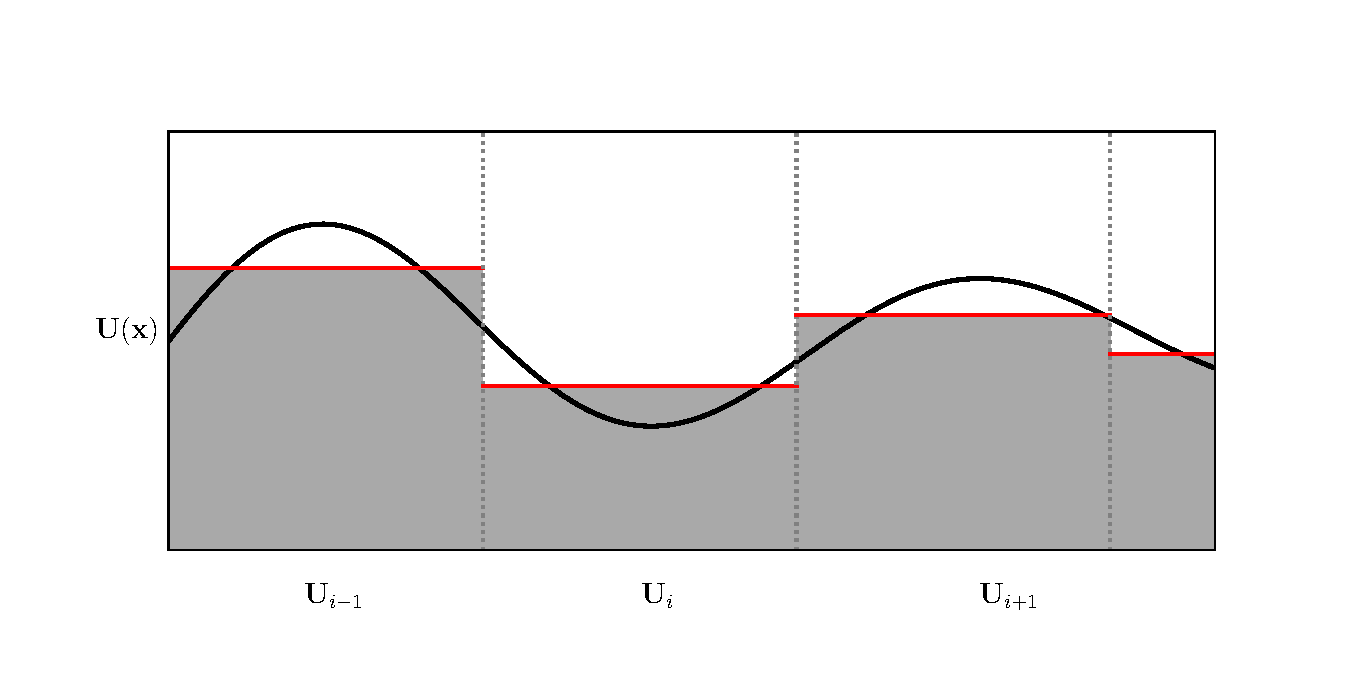
\includegraphics[width=\textwidth]{./images/piecewise_const.pdf}%
	\caption{Piecewise constant reconstruction of the field
		\label{fig:pwconst}
	}
\end{figure}


We assume that the cell state within a cell is constant (fig. \ref{fig:pwconst}).
Furthermore, we also assume that the velocity $\V$ is constant and positive.


\begin{align}
	\U_i ^{n+1} &= 
		\U_i^{n} +  \frac{\Delta t}{\Delta x} \left( \F_{i-\half}^{n+\half} - \F_{i+\half}^{n+\half} \right) \label{eq:advection_basic}\\ 
	\F_{i\pm\half}^{n+\half} &= \V_{i\pm\half}\cdot \U_{i - \half \pm \half} \label{eq:advection_flux}
\end{align}

The method is first order accurate in time and space.





We assumed that the velocity is positive and constant.
What if it's negative?

The important point is that we always do \textbf{downwind differencing}.
To obtain a finite difference, as we do here, you must never use the value that is downstream, i.e. that is in the direction of the flux.
Doing this means taking a value for your computation that won't be valid as soon as an infinitesimal time interval passes, because the ingoing flux will change the downwind state.
This is unphysical and leads to violent instabilites.

So if we have negative velocity, all we need to do is change the expression \ref{eq:advection_flux} to

\begin{equation}
	\F_{i\pm\half}^{n+\half} = \V_{i\pm\half}\cdot \U_{i + \half \pm \half}
\end{equation}









\subsection{Piecewise Linear Method}

\begin{figure}[htbp]
	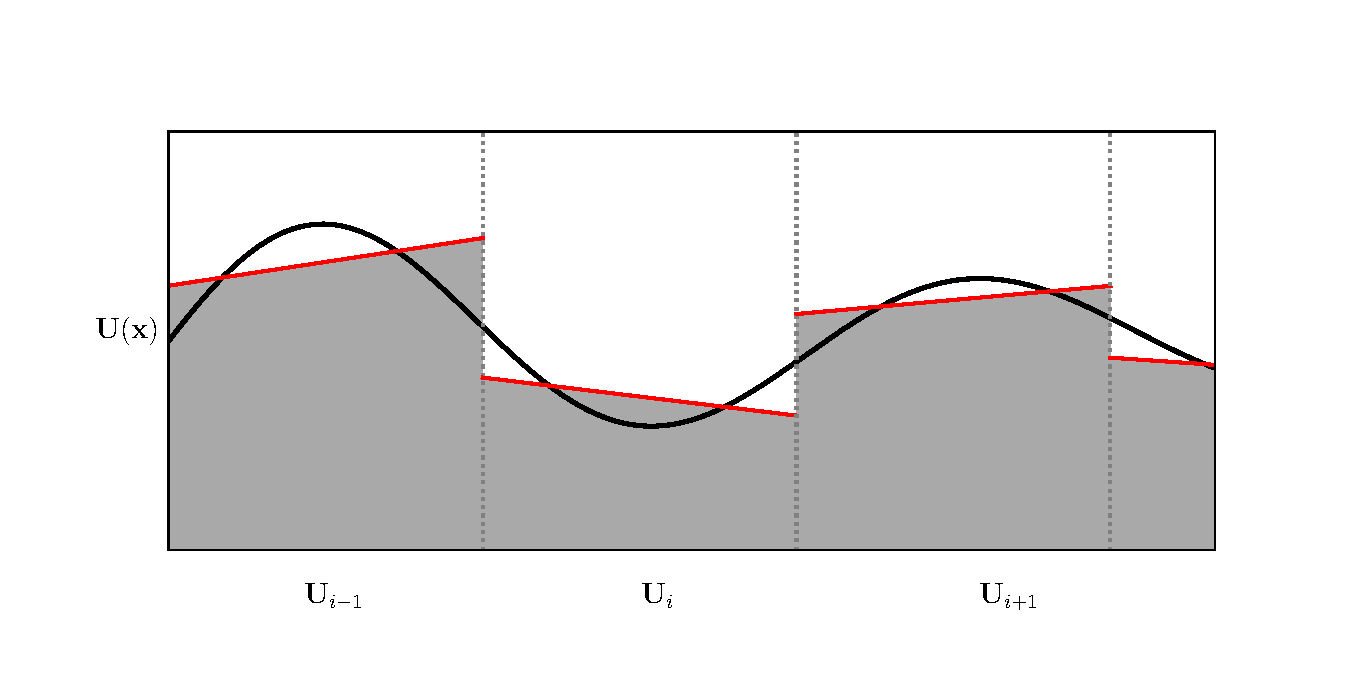
\includegraphics[width=\textwidth]{./images/piecewise_linear.pdf}%
	\caption{Piecewise linear reconstruction of the field
		\label{fig:pwlin}
	}
\end{figure}



This time, we assume that the state is not constant within a cell, but follows a piecewise linear profile with some slope $\mathbf{s}$ (fig. \ref{fig:pwlin}):

\begin{align*}
	\text{For } \x_{i-\half} < \x_i < \x_{i+\half}: &&
	\quad \U(\x, t=t_n) &= \U_i^n + \mathbf{s}_i^n(\x - \x_i) \\
	\text{Centered method:} && \mathbf{s_i}^n &= \frac{\U_{i+1}^n - \U_{i-1}^n}{ 2 \Delta x}
\end{align*}

Other choices for the slope are possible and stable.




Assuming a positive constant velocity $\V$, we derive the flux $\F$ at the time $t^n < t < t^{n+1}$ at the interface position $i-\half$.
At time $t$, the cell will have been advected by a distance $\V (t - t^n)$, and the the current state at the interface will be

\begin{align*}
	\U(x=x_{i-\half}, t) 
		&= \U_{i-1}^n + \mathbf{s}_{i-1} (\x_{i-\half} - \V (t - t^n) - \x_{i-1}) \\
		&= \U_{i-1}^n + \mathbf{s}_{i-1} (\half \Delta x - \V (t - t^n))
\end{align*}

To understand how the $\x_{i-\half} - \V (t - t^n)$ comes into play, imagine the state doesn't change (i.e. isn't advected), but you move the boundaries to the left instead over a distance $\V(t - t^n)$.

So if we have a \textbf{negative} constant velocity, the term changes to 

\begin{align*}
	\U(x=x_{i-\half}, t) 
		&= \U_{i}^n + \mathbf{s}_{i} (\x_{i-\half} - \V (t - t^n) - \x_{i}) \\
		&= \U_{i}^n + \mathbf{s}_{i} (-\V (t - t^n) - \Delta x)
\end{align*}



Note that the minus sign remains, and that the indices changed by one because we need to always make sure to do upwind differencing, i.e. take only values where the flow comes from, not from the direction where it's going.

Finally, we can compute the average flux over the time step $\Delta t = t^{n+1} - t^{n}$:
\begin{align}
	\F_{i-\half}^{n+\half} 
	&= \langle \F_{i+\half}(t)\rangle _{t^n} ^ {t^{n+1}} 
	= \frac{1}{\Delta t} \int_{t^n}^{t^{n+1}} \V \U(\x 
	= \x_{i-\half}, t) \\
	&= \frac{1}{\Delta t} \int_{t^n}^{t^{n+1}} \V \left( \U_{i-1}^n + \mathbf{s}_{i-1} (\half \Delta x - \V (t - t^n)) \right) \\
	&= \V \left( \U_{i-1}^n  + \mathbf{s}_{i-1} \left( \half \Delta x - \V \left( \left[ \frac{1}{2 \Delta t} t^2 \right]_{t^n}^{t^{n+1}} - t^n \right)  \right) \right) \\
	&= \V \left( \U_{i-1}^n  + \mathbf{s}_{i-1} \left( \half \Delta x - \V \left[ \frac{1}{2} (t^{n+1} + t^n) - t^n \right] \right) \right) \\
	&= \V \left( \U_{i-1}^n  + \half \mathbf{s}_{i-1} \left(\Delta x - \V \Delta t \right) \right)
\end{align}



Finally averaging the fluxes over a time step gives:
\begin{equation}
	\U_i^{n+1} = \U_i^n - \V \cdot \frac{\Delta t}{\Delta x} ( \U_i ^n - \U_{i-1}^n) - \V \cdot \frac{\Delta t}{\Delta x} \frac{1}{2} (\mathbf{s}_i^n - \mathbf{s}_{i-1}^n)(\Delta x - \V \Delta t)
\end{equation}

This is the same as eq. \ref{eq:advection_basic} where we used
\begin{align*}
	\F_{i + \half}^{n+\half} 
		& = \V_{i+\half} \cdot  \U_{i+\half} ^{n + \half} \\
		& = \V \cdot \U(\x_{i+\half} - \half \V \Delta t) \\
		& = \V \cdot \left( \U_i^n + \mathbf{s}_i^n [(\x_{i+\half} - \half \V \Delta t) - \x_i ]  \right)\\
		& = \V \cdot \left( \U_i^n + \half \mathbf{s}_i^n (\Delta \x -  \V \Delta t)  \right)\\
\end{align*}

and analoguely
\begin{align*}
	\F_{i - \half}^{n+\half} 
		& = \V \cdot \left( \U_{i-1}^n + \frac{1}{2} \mathbf{s}_{i-1}^n (\Delta \x -  \V \Delta t)  \right)\\
\end{align*}








To summarize the formulae:

\begin{align*}
	\U_i ^{n+1} &= 
		\U_i^{n} +  \frac{\Delta t}{\Delta x} \left( \F_{i-\half}^{n+\half} - \F_{i+\half}^{n+\half} \right) & \\
	\F_{i-\half}^{n+\half} &= 
		\begin{cases}
			\V_{i-\half} \cdot \U_{i-1}^n +  \frac{1}{2} \V_{i-\half} \cdot\mathbf{s}_{i-1}^n (\Delta \x -  \V_{i-\half} \Delta t)
			 	& \quad \text{for } \V \geq 0 \\
			\V_{i-\half} \cdot \U_{i}^n -\frac{1}{2} \V_{i-\half} \cdot \mathbf{s}_{i}^n (\Delta \x + \V_{i-\half} \Delta t)
				& \quad \text{for } \V \leq 0 \\
		\end{cases} \\
	\F_{i+\half}^{n+\half} &= 
		\begin{cases}
			\V_{i+\half} \cdot \U_{i}^n +  \frac{1}{2} \V_{i+\half} \cdot\mathbf{s}_{i}^n (\Delta \x -  \V_{i+\half} \Delta t)
			 	& \quad \text{for } \V \geq 0 \\
			\V_{i+\half} \cdot \U_{i+1}^n -\frac{1}{2} \V_{i+\half} \cdot \mathbf{s}_{i+1}^n (\Delta \x + \V_{i+\half} \Delta t)
				& \quad \text{for } \V \leq 0 \\
		\end{cases} \\		
\end{align*}





We can now insert a more general expression for the slopes.
Let 
\begin{align}
	\theta_{i-\half} = \begin{cases} +1 \quad \text{ for } \V \geq 0 \\ -1 \quad  \text{ for } \V \leq{0} \end{cases}
\end{align}

Then

\begin{align}
	\Delta x_{i-\{0, 1\}} \mathbf{s}_{i-\{0,1\}} 
		&= \frac{1}{2} \Delta x \left[ (1 + \theta_{i-\half}) \mathbf{s}_{i-1}^n + (1 - \theta_{i-\half})  \mathbf{s}_{i}^n \right]  \\
	&\equiv \phi(r_{i-\half}^n) (\U_i^n - \U_{i-1}^n ) \\
	r^n_{i-\half} &= \begin{cases}
		\frac{\U_{i-1}^n - \U_{i-2}^n}{\U_{i}^n - \U_{i-1}^n} 	\quad \text{ for } \V  \geq 0 \\
		\frac{\U_{i+1}^n - \U_{i}^n}{\U_{i}^n - \U_{i-1}^n} 	\quad \text{ for } \V  \leq 0 \\
	\end{cases} 
\end{align}

$\phi$ is discussed later. Finally:

\begin{align}
	\F_{i-\half}^{n+\half} = 
		&\frac{1}{2} \V_{i-\half} \left[  (1 + \theta_{i-\half}) \U_{i-1}^n + (1 - \theta_{i-\half})  \U_{i}^n \right] +\nonumber\\
		&\frac{1}{2}| \V_{i-\half} | \left( 1 - \left| \frac{\V_{i-\half} \Delta t}{\Delta x} \right| \right) \phi(r_{i-\half}^n) (\U_i^n - \U_{i-1}^n ) \label{eq:advection_phi1}\\
	\F_{i+\half}^{n+\half} = 
		&\frac{1}{2} \V_{i+\half} \left[  (1 + \theta_{i+\half}) \U_{i}^n + (1 - \theta_{i+\half})  \U_{i+1}^n \right] +\nonumber\\
		&\frac{1}{2}| \V_{i+\half} | \left( 1 - \left| \frac{\V_{i+\half} \Delta t}{\Delta x} \right| \right) \phi(r_{i+\half}^n) (\U_{i+1}^n - \U_{i}^n ) \label{eq:advection_phi2}
\end{align}







Depending on our choice of $\phi$, we can get different slopes. Here for positive velocity only, and for $r = r_{i-\half}$:

\begin{align*}
	\phi(r) & = 0 \rightarrow \mathbf{s}_i = 0 
		&\text{ No slopes; Piecewise constant method.}\\
	\phi(r) & = 1 \rightarrow \mathbf{s}_i = \frac{\U_{i} - \U_{i-1}}{\Delta x} 
		&\text{ Downwind slope (Lax-Wendroff)} \\
	\phi(r) & = r \rightarrow \mathbf{s}_i = \frac{\U_{i-1} - \U_{i-2}}{\Delta x} 
		&\text{Upwind slope (Beam-Warming)} \\
	\phi(r) & = \frac{1}{2} (1 + r) \rightarrow \mathbf{s}_i = \frac{\U_{i} - \U_{i-2}}{2 \Delta x} 
		&\text{ Centered slope (Fromm)} \\
\end{align*}

















\subsection{CFL Condition}

To keep things stable and physical, we must not allow any flux in the simulation to go further than one single cell size.
Otherwise, you're skipping interactions between fluxes on cells.
This time restriction is known as the CFL condition.

In 1D, it's straightforward:

\begin{equation}
	\Delta t_{max} = C_{cfl} \frac{\Delta x}{v_{max}} \label{eq:CFL1D}
\end{equation}

$C_{cfl} \in [0, 1) $ is a user-set factor.
The lower it is, the more precise the results, but the more computations you need to do.

In 2D, it is:
\begin{equation}
	\Delta t_{max} = C_{cfl} \left( \frac{|v_{x,max}|}{\Delta x} +  \frac{|v_{y,max}|}{\Delta y} \right)^{-1} \label{eq:CFL2D}
\end{equation}

This condition is more strict than what one would expect from the restriction based on physical arguments, i.e. not allowing the flux to pass more than one cell, which would be $\Delta t_{max} = C_{cfl} \min \left\{ \frac{\Delta x}{|v_{x,max}|} ,  \frac{\Delta y}{|v_{y,max}|} \right\} $.
It follows from a convergence condition in (von Neumann) stability analysis of the method.

For $N$ dimensions, the condition translates to

\begin{equation}
	\Delta t_{max} = C_{cfl} \left( \sum_{i=1}^{N} \frac{|v_{i,max}|}{\Delta x_i} \right)^{-1}  \label{eq:CFLND}
\end{equation}